%%
%% This is file `sample-sigconf.tex',
%% generated with the docstrip utility.
%%
%% The original source files were:
%%
%% samples.dtx  (with options: `all,proceedings,bibtex,sigconf')
%% 
%% IMPORTANT NOTICE:
%% 
%% For the copyright see the source file.
%% 
%% Any modified versions of this file must be renamed
%% with new filenames distinct from sample-sigconf.tex.
%% 
%% For distribution of the original source see the terms
%% for copying and modification in the file samples.dtx.
%% 
%% This generated file may be distributed as long as the
%% original source files, as listed above, are part of the
%% same distribution. (The sources need not necessarily be
%% in the same archive or directory.)
%%
%%
%% Commands for TeXCount
%TC:macro \cite [option:text,text]
%TC:macro \citep [option:text,text]
%TC:macro \citet [option:text,text]
%TC:envir table 0 1
%TC:envir table* 0 1
%TC:envir tabular [ignore] word
%TC:envir displaymath 0 word
%TC:envir math 0 word
%TC:envir comment 0 0
%%
%% The first command in your LaTeX source must be the \documentclass
%% command.
%%
%% For submission and review of your manuscript please change the
%% command to \documentclass[manuscript, screen, review]{acmart}.
%%
%% When submitting camera ready or to TAPS, please change the command
%% to \documentclass[sigconf]{acmart} or whichever template is required
%% for your publication.
%%
%%
\documentclass[manuscript,review,anonymous]{acmart}
%%
%% \BibTeX command to typeset BibTeX logo in the docs
\AtBeginDocument{%
  \providecommand\BibTeX{{%
    Bib\TeX}}}

% CUSTOMIZED PACKAGES
% \usepackage{amsmath,amsfonts}
\usepackage{multirow}
\usepackage{adjustbox}
% \usepackage{amssymb}
\usepackage[breakable]{tcolorbox}
\usepackage{booktabs}
\usepackage[table]{xcolor}

%% Rights management information.  This information is sent to you
%% when you complete the rights form.  These commands have SAMPLE
%% values in them; it is your responsibility as an author to replace
%% the commands and values with those provided to you when you
%% complete the rights form.
\setcopyright{acmlicensed}
\copyrightyear{2018}
\acmYear{2018}
\acmDOI{XXXXXXX.XXXXXXX}
%% These commands are for a PROCEEDINGS abstract or paper.
\acmConference[Conference acronym 'XX]{Make sure to enter the correct
  conference title from your rights confirmation email}{June 03--05,
  2018}{Woodstock, NY}
%%
%%  Uncomment \acmBooktitle if the title of the proceedings is different
%%  from ``Proceedings of ...''!
%%
%%\acmBooktitle{Woodstock '18: ACM Symposium on Neural Gaze Detection,
%%  June 03--05, 2018, Woodstock, NY}
\acmISBN{978-1-4503-XXXX-X/2018/06}


%%
%% Submission ID.
%% Use this when submitting an article to a sponsored event. You'll
%% receive a unique submission ID from the organizers
%% of the event, and this ID should be used as the parameter to this command.
%%\acmSubmissionID{123-A56-BU3}

%%
%% For managing citations, it is recommended to use bibliography
%% files in BibTeX format.
%%
%% You can then either use BibTeX with the ACM-Reference-Format style,
%% or BibLaTeX with the acmnumeric or acmauthoryear sytles, that include
%% support for advanced citation of software artefact from the
%% biblatex-software package, also separately available on CTAN.
%%
%% Look at the sample-*-biblatex.tex files for templates showcasing
%% the biblatex styles.
%%

%%
%% The majority of ACM publications use numbered citations and
%% references.  The command \citestyle{authoryear} switches to the
%% "author year" style.
%%
%% If you are preparing content for an event
%% sponsored by ACM SIGGRAPH, you must use the "author year" style of
%% citations and references.
%% Uncommenting
%% the next command will enable that style.
%%\citestyle{acmauthoryear}


%%
%% end of the preamble, start of the body of the document source.
\begin{document}

%%
%% The "title" command has an optional parameter,
%% allowing the author to define a "short title" to be used in page headers.
\title{Easy to Know but Hard to Do? Evolve-and-Adapt for Scientific Research}

%%
%% The "author" command and its associated commands are used to define
%% the authors and their affiliations.
%% Of note is the shared affiliation of the first two authors, and the
%% "authornote" and "authornotemark" commands
%% used to denote shared contribution to the research.
% \author{Ben Trovato}
% \authornote{Both authors contributed equally to this research.}
% \email{trovato@corporation.com}
% \orcid{1234-5678-9012}
% \author{G.K.M. Tobin}
% \authornotemark[1]
% \email{webmaster@marysville-ohio.com}
% \affiliation{%
%   \institution{Institute for Clarity in Documentation}
%   \city{Dublin}
%   \state{Ohio}
%   \country{USA}
% }

% \author{Lars Th{\o}rv{\"a}ld}
% \affiliation{%
%   \institution{The Th{\o}rv{\"a}ld Group}
%   \city{Hekla}
%   \country{Iceland}}
% \email{larst@affiliation.org}

% \author{Valerie B\'eranger}
% \affiliation{%
%   \institution{Inria Paris-Rocquencourt}
%   \city{Rocquencourt}
%   \country{France}
% }

% \author{Aparna Patel}
% \affiliation{%
%  \institution{Rajiv Gandhi University}
%  \city{Doimukh}
%  \state{Arunachal Pradesh}
%  \country{India}}

% \author{Huifen Chan}
% \affiliation{%
%   \institution{Tsinghua University}
%   \city{Haidian Qu}
%   \state{Beijing Shi}
%   \country{China}}

% \author{Charles Palmer}
% \affiliation{%
%   \institution{Palmer Research Laboratories}
%   \city{San Antonio}
%   \state{Texas}
%   \country{USA}}
% \email{cpalmer@prl.com}

% \author{John Smith}
% \affiliation{%
%   \institution{The Th{\o}rv{\"a}ld Group}
%   \city{Hekla}
%   \country{Iceland}}
% \email{jsmith@affiliation.org}

% \author{Julius P. Kumquat}
% \affiliation{%
%   \institution{The Kumquat Consortium}
%   \city{New York}
%   \country{USA}}
% \email{jpkumquat@consortium.net}

%%
%% By default, the full list of authors will be used in the page
%% headers. Often, this list is too long, and will overlap
%% other information printed in the page headers. This command allows
%% the author to define a more concise list
%% of authors' names for this purpose.
% \renewcommand{\shortauthors}{Trovato et al.}

%%
%% The abstract is a short summary of the work to be presented in the
%% article.
\begin{abstract}
Scientific research is a complex process that drives innovation and knowledge advancement. Automating research tasks can reduce researchers' workload and accelerate discovery, but long-horizon planning and execution introduce challenges such as error accumulation and misalignment with human intent. We present Evolve-and-Adapt, a framework that organizes AI research assistants to collaborate with human researchers throughout the research process. In this framework, imitation agents retrieve and emulate reference plans from external sources based on the human researcher's initial idea. Evolution agents use various tools to gather new observations and iteratively refine the plan during execution, guided by human feedback and approval. By integrating imitation and evolution, the AI assistant team automates research tasks while staying aligned with human intent, leading to faithful and desirable outcomes. Experiments show that our framework improves the quality of generated research papers, as measured by review ratings.
\end{abstract}

%%
%% The code below is generated by the tool at http://dl.acm.org/ccs.cfm.
%% Please copy and paste the code instead of the example below.
%%
\begin{CCSXML}
<ccs2012>
   <concept>
       <concept_id>10010147.10010178.10010199.10010202</concept_id>
       <concept_desc>Computing methodologies~Multi-agent planning</concept_desc>
       <concept_significance>500</concept_significance>
       </concept>
   <concept>
       <concept_id>10010147.10010178.10010179.10010182</concept_id>
       <concept_desc>Computing methodologies~Natural language generation</concept_desc>
       <concept_significance>500</concept_significance>
       </concept>
 </ccs2012>
\end{CCSXML}

\ccsdesc[500]{Computing methodologies~Multi-agent planning}
\ccsdesc[500]{Computing methodologies~Natural language generation}

%%
%% Keywords. The author(s) should pick words that accurately describe
%% the work being presented. Separate the keywords with commas.
\keywords{Imitation-and-Evolve, Long-Horizon Planning, Research Paper Generation}
%% A "teaser" image appears between the author and affiliation
%% information and the body of the document, and typically spans the
%% page.
% \begin{teaserfigure}
%   \includegraphics[width=\textwidth]{sampleteaser}
%   \caption{Seattle Mariners at Spring Training, 2010.}
%   \Description{Enjoying the baseball game from the third-base
%   seats. Ichiro Suzuki preparing to bat.}
%   \label{fig:teaser}
% \end{teaserfigure}

% \received{20 February 2007}
% \received[revised]{12 March 2009}
% \received[accepted]{5 June 2009}

%%
%% This command processes the author and affiliation and title
%% information and builds the first part of the formatted document.
\maketitle

\section{Introduction}
Scientific research plays an important role in driving innovation, advancing knowledge, solving problems, expanding our understanding of the world, and ultimately improving people's lives in tangible ways \cite{wang2023scientific}. However, the research process is labor-intensive, requiring researchers to read and synthesize overwhelming amounts of knowledge from a vast and rapidly growing scientific literature in order to formulate research ideas and design corresponding experiments \cite{hope2023computational}. As a result, many promising ideas are often abandoned or overlooked due to the substantial effort needed to identify and validate them.

Automating scientific discovery has been a long-standing ambition in the research community, with early explorations tracing back to the 1970s and 1980s \cite{langley1987scientific}. The recent emergence of large language models (LLMs) \cite{achiam2023gpt} has driven remarkable progress in processing, organizing, and generating scientific text \cite{wang2023scientific}. Increasing efforts now leverage commercial LLMs to develop research agents that can propose novel research ideas \cite{wang2023scimon,yang2024large,baek2025researchagent}, assist in designing and conducting experiments \cite{du2024llms}, or function as AI scientists capable of generating complete, open-ended scientific publications automatically \cite{lu2024ai,yamada2025ai}. State-of-the-art systems further permit closing the loop by automating the entire research and review cycle, including literature review, manuscript drafting, peer review, and iterative paper refinement \cite{weng2025cycleresearcher}.

Recent progress has pushed the boundary to the point where a workshop paper written entirely by AI has been accepted through peer review \cite{yamada2025ai}. However, as highlighted by human evaluations of generated manuscripts \cite{yamada2025ai}, current systems still struggle to produce drafts that are technically sound, well-organized, and clearly written, especially when addressing novel research problems or methods not well represented in existing literature. One of the most challenging bottlenecks leading to these problems is error accumulation in long-horizon planning. Drafting a research paper is inherently a long-horizon task, involving multiple stages of reasoning from literature review and manuscript preparation to peer review and paper refinement. Prior studies on multi-step models have shown that such long-horizon planning inevitably introduces the risk of compounding errors: small mistakes made in early steps can accumulate and propagate through subsequent planning stages, as errors at one stage directly impact downstream decisions \cite{wang2025expressive, han2023expert, venkatraman2015improving, hejna2023improving}.

As a demonstration, we employ state-of-the-art research assistants, OpenAI's Deep Research \cite{openai2025gpt41} and Gemini Deep Research, to draft a paper on Diffusion models for data augmentation in EEG (electroencephalogram)-based emotion recognition. We observe that similar issues exist in the outputs of both Deep Research systems. For example, the planned survey section lacks relevant literature in the retrieved results, resulting in missing citations and hallucinated related work. The proposed method is constructed on top of these hallucinated references, lacking a solid technical foundation. Furthermore, the experimental setting employs inappropriate datasets, which further undermines the validity of the research plan.

Based on these observations, a question arises: How can we mitigate error accumulation in long-horizon planning for scientific research generation? We find that if a plan cannot effectively incorporate new observations, there is a persistent risk of misalignment between the plan and the actual observations. It is hard to anticipate potential observations in advance if possible. Even expert researchers rarely plan and execute an entire research project without making revisions. Instead, they continuously track new results and iteratively realign their ideas with emerging evidence throughout the research process.

In this paper, we propose an Imitation-and-Evolve Multi-agent framework to address the challenge of error accumulation in long-horizon planning for scientific research generation. The contributions of our framework are threefold. (1) We are the first to introduce a multi-agent framework to mitigate error accumulation in long-horizon planning for scientific research generation. The proposed framework employs imitation agents to retrieve reference plans from external sources and evolve agents to utilize tools and derive observations. Based on these observations, the plan is continuously updated during execution. (2) We integrate the imitation-and-evolve paradigm into research lifecycle and propose the first self-improving scientific research generation system. In the research stage, the imitation agent emulates related work to plan the manuscript outline, while the evolve agent iteratively drafts and refines this outline. In the revision, the imitation agent simulates human review to generate a revision plan, and the evolve agent iteratively revises the manuscript and decides whether to adopt each suggestion. (3) We propose a new human–computer interaction paradigm that gives users control over the planning process in scientific research generation, enabling them to steer research outputs according to their preferences. Experiments demonstrate that our approach achieves higher reviewer scores on a public benchmark dataset \cite{weng2025cycleresearcher} and a self-constructed dataset.

\section{Related Work}

\subsection{Large Language Models for Research}

In recent years, several studies have explored the use of language models for creative tasks in research, such as multi-agent collaborative writing~\cite{baek2025researchagent} and multi-module retrieval~\cite{yang2024large} to improve research idea generation. These works aim to enhance the novelty and diversity of artificial intelligence in creative research tasks. Si et al.~\cite{si2024can} conducted a comprehensive human evaluation of idea generation by language models. Wang et al.~\cite{wang2024autosurvey} proposed a method that uses large language models to automatically write survey papers. Additionally, large language models have been applied to automate the research process. For example, Huang et al.~\cite{huang2024mlagentbench} introduced a benchmark for evaluating large language models in coding solutions for machine learning problems. Wang et al.~\cite{wang2023scimon} proposed an approach that leverages large language models for scientific literature retrieval. The AI Scientist project~\cite{lu2024ai} introduced a fully automated, prompt-driven research pipeline. Subsequently, the AI Scientist-v2 project~\cite{yamada2025ai} introduced a workshop-level automated scientific discovery method based on agentic tree search. More recently, Weng et al.~\cite{weng2025cycleresearcher} developed an iterative self-rewarding framework that enables large language models to continuously refine their ideas, thereby enhancing both the diversity and practicality of research proposal generation. Guo et al.~\cite{guo2025ideabench} proposed a benchmark for evaluating large language models in research idea generation. Pu et al.~\cite{pu2025ideasynth} proposed a method for iterative research idea development by evolving and composing idea facets with literature-grounded feedback. Garikaparthi et al.~\cite{garikaparthi2025iris} proposed an interactive research ideation system to accelerate scientific discovery.

Existing work has made progress in research paper generation. However, most approaches rely on predefined or one-shot planning, which risks error accumulation and misalignment between the plan and the actual evidence.

\subsection{Planning of Large Language Model Agents}

Large language models have achieved remarkable success across various domains, demonstrating significant abilities in reasoning, tool usage, planning, and instruction following. The intelligence of large language models highlights their potential as the cognitive core of agents, which offers opportunities to improve planning ability~\cite{huang2024understanding}. For example, Plan-and-Solve~\cite{wang2023plan} proposes a two-step prompt instruction, where the model first devises a plan and then carries out the plan. This zero-shot approach has achieved improvements in mathematical reasoning, common-sense reasoning, and symbolic reasoning. ProgPrompt~\cite{singh2023progprompt} translates natural language descriptions of tasks into coding problems by symbolizing the agent’s action space and objects in the environment through code, with each action formalized as a function and each object represented as a variable. Plan-Act~\cite{erdogan2025planact} targets HTML manipulation, and LLMCompiler~\cite{kim2024llm} breaks down question-answering tasks into parallel execution graphs.

Despite these promising contributions, large language models still fall short in more complex scenarios such as long-horizon planning~\cite{chen2024can}. Several hierarchical planning frameworks have been proposed. AgentOccam~\cite{yangagentoccam} incorporates planning into the action space using tree-like planning. WebPilot~\cite{zhang2025webpilot} uses six different agents. AdaPlanner~\cite{sun2023adaplanner} employs InPlan and Out-of-Plan Refiners for replanning, and ADaPT~\cite{prasad2024adapt} uses recursive decomposition. PLAN-AND-ACT~\cite{erdogan2025plan} provides a two-agent framework with a systematic approach to generating high-quality training data for open-source large language models.

However, although research on planning with large language models has made significant progress, there is still a lack of studies on long-horizon planning, especially for research paper generation.

\section{Methodology}

\begin{figure*}[h]
  \begin{center}
      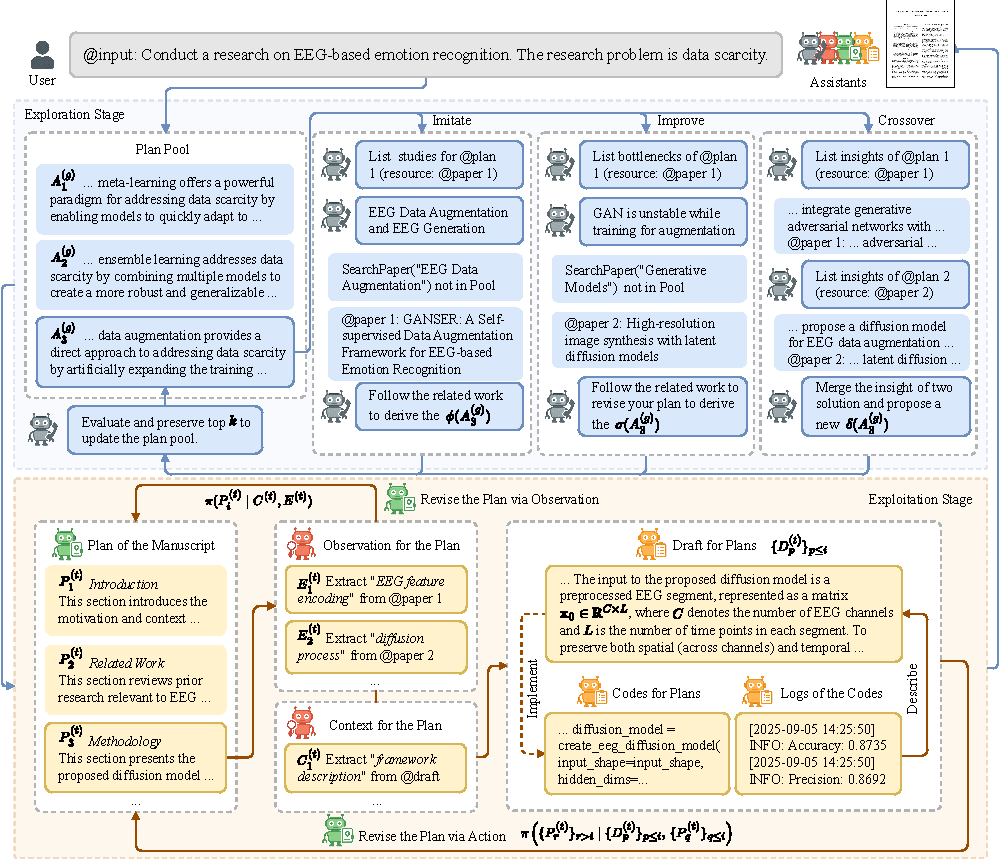
\includegraphics[width=\linewidth]{./framework.pdf}
  \end{center}
  \caption{Overview of the Imitation-and-Evolve framework.}
  \label{fig:framework}
\end{figure*}

In this section, we present our Imitation-and-Evolve approach in detail. The overall framework, illustrated in Fig.~\ref{fig:framework}, consists of two stages: drafting and revision. In the drafting stage, the imitation agent emulates relevant work to plan the manuscript outline, while the evolve agent iteratively drafts and refines the outline. In the revision stage, the imitation agent simulates human review to generate revision plan, and the evolve agent iteratively revises the manuscript and decides whether to adopt each point.

\subsection{Imitation-and-Evolve for Drafting}

Given a user request $U$ describing a research topic, we first propose an imitation agent to imitate human expert planning. The imitation agent first prompts an LLM to analyze $U$ and decompose it into an algorithm of interest $U_A$ and an application of interest $U_T$. Formally, we represent this as $\mu(U) = (U_A, U_T; r)$, where $\mu(.)$ is the decomposition function and $r$ denotes any additional requirements or constraints.

Then, the imitation agent retrieves related work in terms of the algorithm of interest and the application of interest. The retrieval results are represented as $\phi(U_A) = \{L_A^{(1)}, \ldots, L_A^{(K)}\}$ and $\phi(U_T) = \{L_T^{(1)}, \ldots, L_T^{(K)}\}$, where $L_A^{(m)}$ and $L_T^{(n)}$ denote the $m$-th and $n$-th retrieved papers, respectively. The imitation agent is equipped with two tools for retrieval, i.e., a search tool and a rerank tool. The search tool receives a query and invokes HuggingFace's paper API\footnote{https://huggingface.co/docs/hub/api} to search for candidate papers. The rerank tool uses the bge-reranker-v2-m3 \cite{chen2024bge} model to encode both the query and the titles and abstracts of the searched papers, and returns the top $K$ most similar results. To find an optimal combination of retrieved algorithm and application, we prompt the LLM to evaluate all pairs of retrieved algorithms and applications, and identify the best-matched pair. This process derives $M_A \in {L_A^{(m)}}$ and $M_T \in {L_T^{(n)}}$, representing the matched algorithm and application papers, respectively.

The imitation agent refers to the section and subsection outlines of these selected papers as human expert plans for organizing the manuscript. We prompt the LLM to extract the sections and subsections along with their summaries from $M_A$ and $M_T$, resulting in $P_A = \sigma(M_A)$ and $P_T = \sigma(M_T)$. Next, the imitation agent imitates these outlines to generate a new outline for the target manuscript, with the algorithm of interest $U_A$, application of interest $U_T$, and any constraints $r$ as additional inputs. The derived outline $P$ serves as the initial plan for drafting the manuscript.

Then, $P$ is handed off to the evolve agent, which is responsible for executing $P$ and updating it whenever discrepancies between the plan and observed results arise. The evolve agent follows an iterative paradigm, starting from step $n = 1$ and adjustment index $t = 1$, which corresponds to the initial execution before any adjustments. The plan at the $t$-th adjustment is denoted as $P^{(t)} = \{P_1^{(t)}, \ldots, P_N^{(t)}\}$, where $N$ is the number of planned steps. For the plan $P_n^{(t)}$ at the $n$-th step after $t-1$ adjustments, the evolve agent first fetches observations relevant to $P_n^{(t)}$. The evolve agent is equipped with two tools, i.e., an external tool for fetching segments from external resources, and a contextual tool for fetching content within the existing draft. When using these tools, the evolve agent is provided with external resources, such as $M_A$ and $M_T$, or the current draft as context. The LLM is prompted to identify the appropriate line ranges, and the content within these ranges is extracted and concatenated to facilitate efficient evidence gathering. The content retrieved from context for step $n$ is denoted as $C_n$, while the content retrieved from external resources is denoted as $E_n$. Using these observations, the evolve agent updates the plan according to

\begin{equation}
P_i^{(t+1)} = \pi(P_i^{(t)} \mid C^{(t)}, E^{(t)}, P_i^{(t)})
\end{equation}
where $\pi(.)$ is a policy function that revises each step $i$ of the current plan based on the available context $C^{(t)}$, external evidence $E^{(t)}$, and the $i$-th step of the current plan $P_i^{(t)}$. The policy function is implemented by prompting the LLM to update the plan according to the observations. Then, the evolve agent 

The revised step $P_i^{(t+1)}$ is then executed to produce the draft $D_i$ for the $i$-th section, using the contextual segments $C_i$ and external segments $E_i$ as context, and $P_i^{(t+1)}$ as the instruction. After deriving the draft $D_i$, the imitation agent further updates the remaining steps in the plan. The subsequent plan steps are modified as needed to be appropriate given the new results:

\begin{equation}
P_j^{(t+2)} = 
\begin{cases}
P_j^{(t)}, & \text{if } j < i \\
P_j^{(t+1)}, & \text{if } j = i \\
\pi\left(P_j^{(t)} \mid \{D_p^{(t)}\}_{p \leq i},\, \{P_q^{(t)}\}_{q < j}\right), & \text{if } j > i
\end{cases}
\end{equation}
where $P_j^{(t+2)}$ denotes the $j$-th step in the updated plan after considering the collection of drafts $\{D^{(t)}_p\}_{p \leq i}$ already produced and the collection of plan steps $\{P_q^{(t)}\}_{q < j}$ as context. In this paper, the LLM is prompted to revise the subsequent plan steps and return a revised version if the current steps are not appropriate; otherwise, the original steps are retained.

Next, the evolve agent moves to the next step in the plan and starts a new round of iteration. This iterative process continues until all $N$ steps are completed. Finally, the evolve agent collects the section titles according to the last version of the plan and combines them with all the drafts $\{D_1, D_2, \ldots, D_N\}$ to form the main body of the manuscript. The evolve agent then prompts the LLM to generate the title and abstract based on the completed body as context. Supplemented with references, all the content is rendered into a LaTeX project according to the conference template, and the final PDF of the paper is generated.

\subsection{Imitation-and-Evolve for Revision}

After deriving draft sections $\{D_1, D_2, \ldots, D_{N_D}\}$, we design the revision stage, which aims to further improve the manuscript. To plan systematic revisions, we introduce an imitation agent that mimics the peer-review and revision process commonly practiced by human experts in scientific research.

We first design the imitation agent to generate review feedback and decompose it into actionable points, which then serve as the revision plan. Following the standard peer-review protocols adopted by leading conferences that make their review comments public on OpenReview\footnote{https://openreview.net/} (e.g., ICLR), our imitation agent prompts the LLM to generate comprehensive review feedback across multiple dimensions. Formally, given the complete manuscript $\{D_1, D_2, \ldots, D_{N_D}\}$, the imitation agent applies a feedback generation function $\delta$ such that $F = \delta(\{D_1, D_2, \ldots, D_{N_D}\})$. The generated feedback $F$ covers aspects such as summary, soundness, presentation, contribution, strengths, weaknesses, questions, and overall rating. Next, we decompose $F$ into a set of review points $\{G_1, G_2, \ldots, G_L\} = \beta(F)$, where $\beta$ is a decomposition function that prompts the LLM to enumerate feedback items from $F$. Each $G_l$ represents a comment that can be addressed independently, forming the initial revision plan.

These review points $\{G_1, G_2, \ldots, G_L\}$ are then handed off to the evolve agent, which is responsible for executing and updating the revision plan in response to observed outcomes. The evolve agent operates in an iterative paradigm, starting from review point $l = 1$ and adjustment index $t = 1$, corresponding to the initial execution before any adjustments. The revision plan at the $t$-th adjustment is denoted as $\{G_1^{(t)}, \ldots, G_L^{(t)}\}$, where $L$ is the total number of review points. For a given review point $G_l^{(t)}$ at step $l$ after $t-1$ adjustments, the evolve agent first gathers relevant observations. Similar to imitation-and-evolve for drafting, it is equipped with two tools: an external tool for retrieving evidence from external resources, and a contextual tool for extracting content from the current manuscript draft. The content extracted from the current draft for step $l$ is denoted as $C_l$, while content from external resources is denoted as $E_l$.

Not all review feedback should be followed unconditionally, as some points may arise from misunderstandings. Therefore, for each plan $G_l$, the evolve agent determines whether to revise or rebut using a decision function $C(G_l, C_l, E_l) \in \{0, 1\}$, where $0$ indicates rebuttal and $1$ indicates revision. The update to the plan before execution can be formalized as:

\begin{equation}
  G_l^{(t+1)} =
  \begin{cases}
    \varnothing, & \text{if } C(G_l, C_l, E_l) = 0 \\
    G_l^{(t)}, & \text{if } C(G_l, C_l, E_l) = 1
  \end{cases}
\end{equation}
where $\varnothing$ denotes an empty plan that does not need to be executed, indicating that the review point is skipped if the decision is to rebut. If the decision is to rebut, the agent skips to the next point. Otherwise, the agent proceeds to modify the relevant section identified by $C_l$. The revised section is denoted as $\hat{D}_i = \eta(D_i, G_l)$, where $\eta$ is a modification function that incorporates the feedback $G_l$ into the original section draft $D_i$.

After executing the plan, we evaluate the revised draft to assess its quality. Here, we prompt the LLM to generate feedback on both versions, putting the revised section $\hat{D}_i$ and the original $D_i$ back into the manuscript, respectively. Then we use $\delta()$ to generate feedback on the two versions of the manuscript and extract a quality score, with the derived score of the corresponding version denoted as $\gamma(\cdot)$. The acceptance or rollback of the update can be formalized as:

\begin{equation}
  D_i^{(t+1)} =
  \begin{cases}
      \hat{D}_i, & \text{if } \gamma(\hat{D}_i) \geq \gamma(D_i) \\
      D_i, & \text{if } \gamma(\hat{D}_i) < \gamma(D_i)
  \end{cases}
\end{equation}
where the revision is accepted only if $\gamma(\hat{D}_i) \geq \gamma(D_i)$, indicating a genuine improvement. If the quality does not improve, we roll back to the previous version, keeping $D_i$ unchanged.

This iterative process continues for all review points $\{G_1, G_2, \ldots, G_L\}$, resulting in a revised draft. The entire revision cycle can be repeated with new rounds of review feedback and revisions.

\section{Conclusion}

In this work, we address the persistent challenge of error accumulation in long-horizon planning for automated scientific research generation. We propose the Evolve-and-Adapt framework, which integrates imitation and evolve agents to continuously realign research plans with new observations, and introduce a novel human–computer interaction paradigm that empowers users to intervene at any stage. Experimental results on both public and self-constructed benchmarks demonstrate that our approach achieves superior reviewer scores compared to state-of-the-art methods.

For future work, we plan to conduct more comprehensive subjective experiments by involving PhD students in human-in-the-loop control and professors in review and evaluation. This will enable us to further assess and enhance the proposed framework in real-world research scenarios.

%%
%% The next two lines define the bibliography style to be used, and
%% the bibliography file.
\bibliographystyle{ACM-Reference-Format}
\bibliography{sample-base}

\end{document}
\endinput
%%
%% End of file `sample-sigconf.tex'.
